\documentclass[tikz,border=10pt]{standalone}
\usepackage{tikz}
\usetikzlibrary{arrows.meta,positioning}

\tikzset{
  card/.style={draw=blue!70!black, line width=1.2pt, rounded corners=3pt, minimum width=6.0cm, minimum height=1.0cm, align=center, fill=none},
  result/.style={draw=orange!80!black, line width=1.2pt, rounded corners=3pt, minimum width=6.0cm, minimum height=1.0cm, align=center, fill=none},
  flow/.style={-{Stealth[length=3mm]}, line width=1.2pt, draw=black!70}
}

\begin{document}
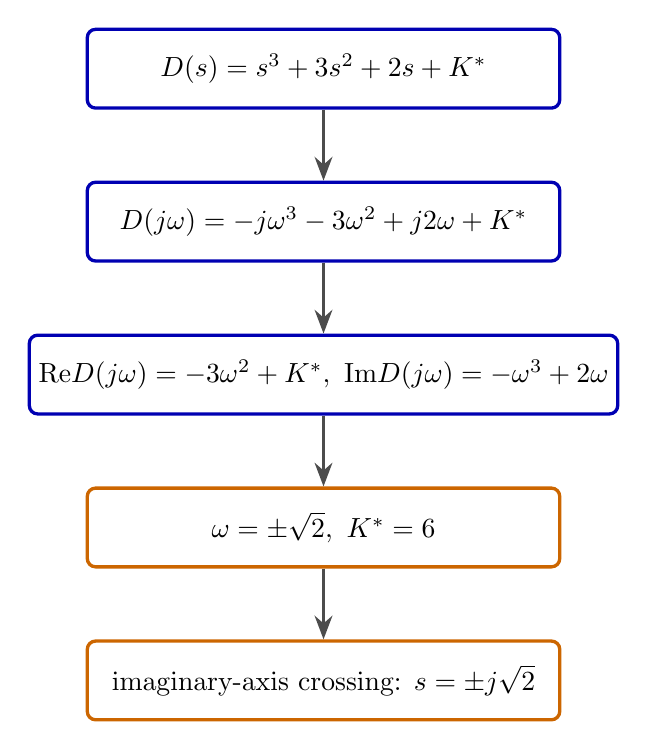
\begin{tikzpicture}[node distance=0.9cm]
  \node[card] (a) {$D(s)=s^3+3s^2+2s+K^\ast$};
  \node[card, below=of a] (b) {$D(j\omega)=-j\omega^3-3\omega^2+j2\omega+K^\ast$};
  \node[card, below=of b] (c) {$\mathrm{Re}D(j\omega)=-3\omega^2+K^\ast,\ \mathrm{Im}D(j\omega)=-\omega^3+2\omega$};
  \node[result, below=of c] (d) {$\omega=\pm\sqrt{2},\ K^\ast=6$};
  \node[result, below=of d] (e) {imaginary-axis crossing: $s=\pm j\sqrt{2}$};

  \draw[flow] (a) -- (b);
  \draw[flow] (b) -- (c);
  \draw[flow] (c) -- (d);
  \draw[flow] (d) -- (e);
\end{tikzpicture}
\end{document}
